% % % % % % % % % % % % % % % % % % % % % % % % % % % % % % % % % % % % %
% Chapter: Experiment 2
% % % % % % % % % % % % % % % % % % % % % % % % % % % % % % % % % % % % %
\chapter{Experiment 2: Smarter values generation}
\label{cpt:experiment2}
% % % % % % % % % % % % % % % % % % % % % % % % % % % % % % % % % % % % %
% Section: Smarter values generation
%\section{Smarter values generation}
%\label{sec:ch4_smarter_values_generation}
\pinfo{Context - result of experiment 1, what aim is now}
Some bugs were found by using random input values in the first experiment. However the implicative properties were not effectively checked in terms of triggering the if-clause when using random input values. This is what we aim to improve in this experiment, expecting to detect more bugs.

% % % % % % % % % % % % % % % % % % % % % % % % % % % % % % % % % % % % %
% Section: Method
\section{Method}
\pinfo{2 categories separation}
We can separate the properties that we have in 2 different categories: those using implication ($\implies$) and those that do not. The defined properties are being separated over two specifications according to which category these belong. We name these specifications \textit{MoneyExpressions} and \textit{MoneyConditionals}. For the \textit{MoneyConditionals} specification (the implicative properties), another way of generating the random values is more useful. The random input values are being optimized such that the condition of the if-clause of these properties are being satisfied. For the other specification (\textit{MoneyExpressions}), the earlier approach (random values as input) can still be used, we do not need to change this functionality for these cases.\\
\\
\pinfo{Adding preconditions}
In the \textit{MoneyConditionals} specification, the condition to trigger the if-clauses will be added to the preconditions of each the event definition, such that these can be used to generate the values matching this clause. The updated event definition of the \textit{Symmetric} property is shown in \autoref{lst:experiment2_updated_definition} for example. Where the preconditions have been added to the event definition.
% Listing
\FloatBarrier
\begin{sourcecode}[!ht]
\begin{lstlisting}[language=Rebel]
event symmetric(x: Money, y:Money) {
    preconditions {
        x == y;
    }
    postconditions {
       new this.result == ( (x == y) ? y == x : False );
    }
}
\end{lstlisting}
\caption{The updated event definition of the \textit{Symmetric} property}
\label{lst:experiment2_updated_definition}
\end{sourcecode}
\FloatBarrier
% End listing
\pinfo{Generating checks for preconditions}
When generating the test suite, the events are being traversed. In case an event with some preconditions is found, it generates a list of value tuples that satisfy the condition to trigger the if-clause. Which is different compared to the generated tests in \autoref{cpt:experiment1}.\\
\\
\pinfo{Diff1: custom generator}
The first difference is that it now uses our custom generator to determine the input values, instead of the built-in Java random generator. A list of tuples, containing values which satisfies the if-clause of the implication, are being generated. Our custom generator is a simple proof of concept in order to check if this will actually result in more failing tests. This custom generator basically consists of multiple methods which are being called based on the event name. In \autoref{lst:ch4_second_generating_values} this behavior is shown for the \textit{Symmetric} and \textit{Division1} event. The \textit{String} parameter of these methods is a way how we can pattern match on the event name in \textit{Rascal}. In case the event couldn't be handled, an exception is thrown.
% Listing
\FloatBarrier
\begin{sourcecode}[!ht]
\begin{lstlisting}[language=Rascal]
private list[Expr] genTestValueForEvent("Symmetric") {
    Expr moneyValue = genRandomMoney();
    return [moneyValue, moneyValue];
}
private list[Expr] genTestValueForEvent("Division1") {
    real moneyAmountX = genRandomDouble();
    real intAmountY = genRandomInteger();
    real moneyAmountZ = moneyAmountX * intAmountY;
    str currency = genRandomCurrency();
    return [convertToMoney(currency, moneyAmountX), converToExpr(intAmountY), convertToMoney(currency, moneyAmountZ)];
}
private default list[Expr] genTestValueForEvent(str eventName) {
    throw "genTestValueForEvent not implemented for event <eventName>";
}
\end{lstlisting}
\caption{Values generation for \textit{Symmetric} and \textit{Division1}, including the fall-back case.}
\label{lst:ch4_second_generating_values}
\end{sourcecode}
\FloatBarrier
% End listing
\pinfo{Not very dynamic}
This means that the way how we determine these values is basically hard-coded, requiring to have knowledge about the if-clause itself. Note that this doesn't make this approach very dynamic, but the result will consist of a list of tuples that satisfy the if-clause. These tuples will be used as input for the test case that will be generated.\\
\\
\pinfo{Mutating values with random operation}
However, the values that are generated now are fixed when we use them directly in a test case, which completely removes the randomness of the values when running the tests. It would be better to keep the randomness, such that the values are different on each run. To solve this problem, we mutate the values in the list such that the values are sort of random again. The tuples still have to satisfy the condition to trigger the if-clause, as this was the actual intention. So the second difference is that for each tuple in the list, we will generate a random operation and use that operation to mutate the values inside the tuple. To ensure that the tuple values still satisfy the condition of the if-clause, each value will be mutated by the same operation. In \autoref{lst:experiment2_second_resulting_test} an example of a generated test case is shown.
% Listing
\FloatBarrier
\begin{sourcecode}[!ht]
\begin{lstlisting}[language=Scala]
"work with Antisymmetry" in {
      Seq((USD(1593.62), USD(1593.62)), (USD(2869.78), USD(2869.78)),
          (EUR(4676.80), EUR(4676.80)), (USD(1850.29), USD(1850.29)),
          // ... // More values in the list
          (USD(9501.16), USD(9501.16)), (- EUR(149.67), - EUR(149.67)),
          (- EUR(159.67), - EUR(159.67)), (EUR(8015.77), EUR(8015.77)))
      .foreach {
        data:  (Money, Money) => {
          val randomOperation = genRandomOperation(genRandomOperator("Money", true), generateRandomMoney(data._1.currency), generateRandomInteger(true), generateRandomInteger(false), generateRandomPercentage(true), generateRandomPercentage(false), Random.nextInt(10))

          checkAction(Symmetry(
              randomOperation(data._1),
              randomOperation(data._2)
              )
          )
        }
      }
    }
\end{lstlisting}
\caption{Resulting test case with semi-random values. Omitted some input tuples for readability.}
\label{lst:experiment2_second_resulting_test}
\end{sourcecode}
\FloatBarrier
% End listing
\pinfo{Small explanation about the new test case}
The list of values are generated by using our custom generator, the amount of tuples in the list can be defined when generating the test suit. A method \code{genRandomOperation()} has been added to the template, which is used to mutate the fixed values in the list. After all the \code{checkAction()} method is being called to check the result of the test.\\
\\
\pinfo{Also: else now returns false}
Now that the input values for the implication events should always satisfy the condition of the if-clause, we can also update the specification such that the else-clause of the expression always returns \textit{False}. This results in a failing case again in case the precondition was not met. When this happens, it could indicate that there's a problem with either our custom generator, or in the generator.

% % % % % % % % % % % % % % % % % % % % % % % % % % % % % % % % % % % % %
% Section: Results
\section{Results}
\pinfo{Failing tests: Division}
Running the test suit with these changes results in 2 additional failing tests compared to the first experiment (\autoref{cpt:experiment1}). An overview of the failing properties and the used input values are shown in \autoref{tbl:experiment2_overview_first_run}. The log of the test run reports that the precondition was not met when using these input values, as shown in \autoref{lst:experiment2_log_first_run}.
% Table
\FloatBarrier
\begin{table}[!ht]
\centering
\begin{tabular}{llll}
\hline
\textbf{Property name} & \textbf{x}    & \textbf{y} & \textbf{z} \\ \hline
Division1              & -16729.90 USD & 830        & -20.16     \\
Division2              & -44.68 USD    & 870        & -38870.47  \\ \hline
\end{tabular}
\caption{Failing tests overview along with its input values}
\label{tbl:experiment2_overview_first_run}
\end{table}
\FloatBarrier
% End table

% Listing
\FloatBarrier
\begin{sourcecode}[!ht]
\begin{lstlisting}[language=Log]
[info] MoneyConditionals
[info] - should work with Additive4params (7 seconds, 224 milliseconds)
[info] - should work with AntisymmetryLET (5 seconds, 493 milliseconds)
[info] - should work with Symmetric (5 seconds, 344 milliseconds)
[info] - should work with Division2 *** FAILED *** (23 milliseconds)
[info]   java.lang.AssertionError: assertion failed: expected CommandSuccess(Division2(-16729.90 USD,830,-20.16 USD)), found CommandFailed(NonEmptyList(PreConditionFailed(x == z*y)))
[info] - should work with Division1 *** FAILED *** (127 milliseconds)
[info]   java.lang.AssertionError: assertion failed: expected CommandSuccess(Division1(-44.68 USD,870,-38870.47 USD)), found CommandFailed(NonEmptyList(PreConditionFailed(x*y == z)))
// ...
\end{lstlisting}
\caption{Precondition failed error in \textit{Division1} and \textit{Division2}.}
\label{lst:experiment2_log_first_run}
\end{sourcecode}
\FloatBarrier
% End listing

% % % % % % % % % % % % % % % % % % % % % % % % % % % % % % % % % % % % %
% Section: Analysis
\section{Analysis}
The values used in the test case should be correct, since we generated these values such that they satisfy the condition of the if-clause and thus they should satisfy the preconditions. Note that the conditions of the if-clause were added as preconditions in the \textit{MoneyConditionals} specification, which causes the error. As the \textit{PreConditionFailed} error is thrown by the system when the input values do not satisfy the preconditions.\\
\\
\pinfo{Describe precision error happening at first}
For \textit{Division1} it states that the condition \code{x*y == z} failed. The
values used for \textit{x}, \textit{y} and \textit{z} were \textit{-44.68 USD},
\textit{870} and \textit{-38870.47 USD} respectively. The result of
\textit{x * y} = \textit{-44.68 USD * 870} = \textit{-38871.60 USD}. This should
be equal to \textit{z}, in fact, the input of \textit{z} was slightly different,
\textit{-38870.47 USD}.\\
\\
Remember that the input values are being mutated by a
random operation that we have added to the test cases. This difference is caused
by the precision error when operating with the \textit{Money} type, which was
found in \autoref{cpt:experiment1}. The random operation that was done was
causing this behaviour. The same goes for the error with \textit{Division2},
where \code{x == z*y} should hold. The values of \textit{x}, \textit{y} and
\textit{z} are \textit{-16729.90 USD}, \textit{830}, \textit{-20.16 USD}
respectively. The result of \textit{z * y} = \textit{-16732.80 USD}, which is
not equal to \textit{-16729.90} USD.\\
\\
\pinfo{Next (when fixed precision), division problem}
The first experiment already described the precision problem and how it could be fixed. To solve this problem, we modify the generator such that the precision error is fixed when generating the system. Then the test framework is being executed again to check whether both tests are succeeding. This resulted in the same amount of tests that were failing, which means that we found a different case now. In \autoref{tbl:experiment2_overview_second_run} an overview of the used input values are shown\footnote{The decimals have been truncated for readability, \autoref{lst:experiment2_log_second_run} shows the exact values}. The log reported that, one case still fails on the precondition check, while the other case just reports values for which the result is \textit{false}, as shown in \autoref{lst:experiment2_log_second_run}.
% Table
\FloatBarrier
\begin{table}[!ht]
\centering
\begin{tabular}{llll}
\hline
\textbf{Property name} & \textbf{x}                               & \textbf{y} & \textbf{z}                               \\ \hline
% Division1              & 1.504347826086956521739130434782609 USD  & -779       & -1171.886956521739130434782608695652 USD \\
Division1              & 1.5043478260... USD     & -779       & -1171.8869565217... USD \\
% Division2              & -3328.825454545454545454545454545455 USD & -129       & 25.80484848484848484848484848484848 USD  \\ \hline
Division2              & -3328.8254545454... USD & -129       & 25.8048484848... USD    \\ \hline
\end{tabular}
\caption{Failing tests overview, after fixing precision errors}
\label{tbl:experiment2_overview_second_run}
\end{table}
\FloatBarrier
% End table

% Listing
\FloatBarrier
\begin{sourcecode}[!ht]
\begin{lstlisting}[language=Log]
[info] MoneyConditionalsSpec:
[info] MoneyConditionals
[info] - should work with Additive4params (7 seconds, 24 milliseconds)
[info] - should work with AntisymmetryLET (3 seconds, 66 milliseconds)
[info] - should work with Symmetric (4 seconds, 361 milliseconds)
[info] - should work with Division2 *** FAILED *** (670 milliseconds)
[info]   java.lang.AssertionError: assertion failed: expected CommandSuccess(Division2(-3328.825454545454545454545454545455 USD,-129,25.80484848484848484848484848484848 USD)), found CommandFailed(NonEmptyList(PreConditionFailed(x == z*y)))
[info] - should work with Division1 *** FAILED *** (316 milliseconds)
[info]   java.lang.AssertionError: assertion failed: expected CurrentState(Result,Initialised(Data(None,Some(true)))), found CurrentState(Result,Initialised(Data(None,Some(false)))): With command: Division1(1.504347826086956521739130434782609 USD,-779,-1171.886956521739130434782608695652 USD)
// ...
\end{lstlisting}
\caption{Precondition failed error in \textit{Division1} and \textit{Division2}.}
\label{lst:experiment2_log_second_run}
\end{sourcecode}
\FloatBarrier
% End listing
\pinfo{Division2 triggers division problem}
The test concerning \textit{Division2} shows that the precondition check fails. If we look at the input values, it can be seen that the \textit{Money} values are a fractional number. As it contains many decimals and it rounds up at the end. When operating with this rounded value, the resulting value is also slightly different. As the generated system is implemented such that the preconditions are being checked first, the \textit{PreConditionFailed} exception is thrown. This leads to the issue of the division problem \todo{Source?} in which a number cannot be equally divided. In \autoref{cpt:properties}, we defined that the precision in this case should be of X \todo{Define X} decimals. However, the test framework does not specifically check for this precision yet.\\
\\
\pinfo{Division1 triggers difference in rounding problem}
% Division1 is defined as \code{x*y == z $\implies$ x == z/y}.
When looking at \textit{Division1}, we see another case as the input values passed the precondition checks. This indicates that the values satisfy the condition to trigger the if-clause of the property. However, the result of the if-clause returns \textit{false}, showing us that the property does not hold when using these input values. Thus a case has been found for which the \textit{Division1} property doesn't hold. The investigation of the intermediate calculation steps are shown in TX. Note that the \textit{Division1} property is defined as \code{x*y == z $\implies$ x == z/y}.

% Table
\FloatBarrier
\begin{table}[!ht]
\centering
\begin{tabular}{rll}
\hline
\textbf{Variable}  & \textbf{Value}                                    & \textbf{Type}                                        \\ \hline
X                  & 1.504347826086956521739130434782609 USD           & Money                                                \\
Y                  & -779                                              & Integer                                              \\
Z                  & -1171.886956521739130434782608695652 USD          & Money                                                \\ \hline
\textbf{Formula}   & \textbf{Scala result}                             & \textbf{Expected result}                             \\ \hline
x*y == z           & true                                              & false                                                \\
x == z/y           & false                                             & false                                                \\
                   &                                                   &                                                      \\
x*y                & -1171.886956521739130434782608695652 USD          & -1171.886956521739130434782608695652\textbf{411} USD \\
z/y                & 1.504347826086956521739130434782608 USD           & 1.504347826086956521739130434782608 USD              \\ \hline
\end{tabular}
\caption{Division1: Difference in rounding}
\label{tbl:experiment2_division1_rounding_difference}
\end{table}
\FloatBarrier
% End table

In the results we can see that the expected values do not match the property either. Although in \textit{Scala} the first expression is considered true. Since the expected results also return false for the intermediate calculations, the input values might not fully satisfy the condition to trigger the if-clause. Which could be an implementation error in our calues generator. However, its notable that in \textit{Scala} the condition is considered to hold, which triggered this case. This indicates that there is a rounding error happening in the system, which triggered this case.\\
\\
Unfortunately, we are unable to trace back how the input values used for this tests were exactly determined. As these are build up by using random generated and then being mutated by a random operation. 




% In conclusion currently:
When defining the properties in \autoref{cpt:properties}, we said that when this problem occurs, the value has to be rounded at the Xth \todo{Define x} decimal. However, these tests reveal that the generated system does not yet take this rule into account. Instead it tries to hold the exact value. As we have seen in Listing X \todo{Add listing}, one case (\textit{Division1}) fails because of a \code{PreconditionFailed} error, while \textit{Division2} passed the precondition check but results in \textit{false}. Since the \textit{Division2} test passes the precondition check in this example, it is probably the case that the calculated value tried to be used. The result check reveals that the property is still failing, meaning that it fails to hold the exact value. Which is understandable, as it has to be rounded somewhere, but it is not defined clearly yet. But this reveals that it is not the case that the rounding is done at the Xth \todo{Define x} decimal according to our definition.

% % % % % % % % % % % % % % % % % % % % % % % % % % % % % % % % % % % % %
% Section: Evaluation criteria
\section{Evaluation criteria}
\pinfo{Property coverage}
When looking at the coverage report concerning a specific property, it can be seen that the else-clause of the implication is not being triggered any more. In \autoref{fig:experiment2_eval_e2_highlighting_transitive-equality} the coverage of \textit{TransitiveEquality} is shown, note that only the else condition (which was translated to \textit{false}) is not triggered by the test suite. This was also the intention of the modification used in this experiment, as the if-clause is actually what we wanted to check in this experiment.
% Figure
\FloatBarrier
\begin{figure}[!ht]
\frame{
	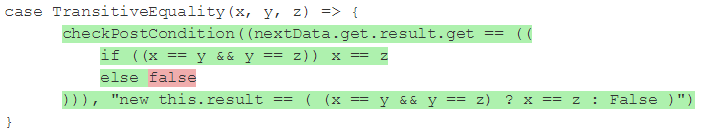
\includegraphics[width=\linewidth]{figures/eval_e2_transitive-equality}
}
\caption{Test coverage for \textit{TransitiveEquality} in second experiment}
\label{fig:experiment2_eval_e2_highlighting_transitive-equality}
\centering
\end{figure}
\FloatBarrier
% End figure

% Evaluation criteria
\pinfo{74\% on conditionals. Others remain the same - image}
The expectation was that the test suite could be improved, such that the test coverage on the SUT would become higher. In the first experiment we found that the properties using implication were not tested thoroughly. In this experiment these properties are triggering the if-clause of the properties using implication, thus we expect the test coverage to be higher when looking on the coverage of the properties. This is also follows from the results, as we can see in \autoref{fig:experiment2_eval_e2}, the test coverage when looking at the logic file of the implicative properties is 74\%.
% Figure
\FloatBarrier
\begin{figure}[!ht]
\frame{
	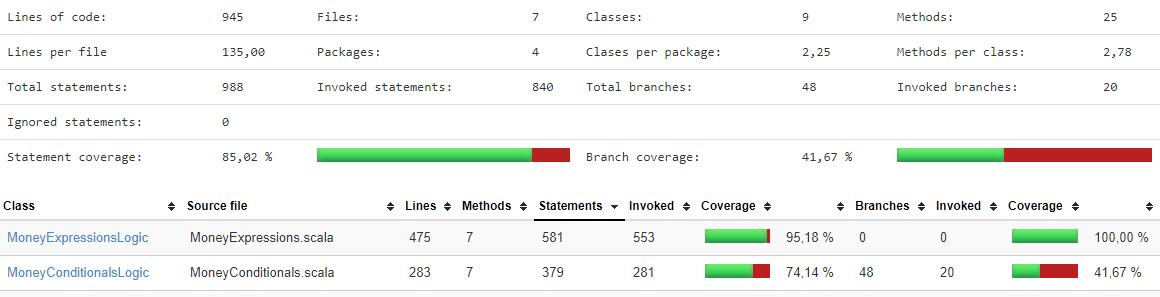
\includegraphics[width=\linewidth]{figures/eval_experiment2}
}
\caption{Test coverage report of the first experiment}
\label{fig:experiment2_eval_e2}
\centering
\end{figure}
\FloatBarrier
% End figure
\pinfo{Coverage, 85\% (overall), better}
The total test coverage on the SUT is reported to be 85\%. As we have discussed in the evaluation of the first experiment, we do not expect to reach the 100\% coverage, as there are certain components in the generated system which we do not test with this approach. Also, considering that the else-clause is not being triggered of the implicative properties, the test coverage will never become 100\%. Which is not a problem in that sense, as we don't intent to test the else clause, we are more interested in the result of the if-clause of these implicative properties.\\
\\
\pinfo{\# of bugs, 2 more}
The other criteria we use was the amount of bugs that we have found. Using this approach 2 more tests were failing compared to the first experiment in \autoref{cpt:experiment1}. The bug found was when using division with the \textit{Money} type, which is expected to be rounded off at the Xth decimal \todo{Define X}. However, as we have seen in this experiment, the generated system does not take this into account. We can categorize this bug into one category, rounding errors. These are different from precision errors as the precision errors are caused by having an incorrectly calculated value, where rounding errors are basically not working with the rounding method that is defined.

% % % % % % % % % % % % % % % % % % % % % % % % % % % % % % % % % % % % %
% Section: Conclusion
\section{Conclusion}
In this experiment we generated the input values such that the condition of the properties using implication are satisfied. Although this did not lead to many additional bugs compared to the earlier experiment, there were still 2 additional failing tests related to the division problem. Both failing tests are related to the division problem that occurs when there is no even division of a number. For example: when dividing 1 by 3.\\
\\
When defining the properties in \autoref{cpt:properties}, we said that when this problem occurs, the value has to be rounded at the Xth \todo{Define x} decimal. However, these tests reveal that the generated system does not yet take this rule into account. Instead it tries to hold the exact value. As we have seen in Listing X \todo{Add listing}, one case (\textit{Division1}) fails because of a \code{PreconditionFailed} error, while \textit{Division2} passed the precondition check but results in \textit{false}. Since the \textit{Division2} test passes the precondition check in this example, it is probably the case that the calculated value tried to be used. The result check reveals that the property is still failing, meaning that it fails to hold the exact value. Which is understandable, as it has to be rounded somewhere, but it is not defined clearly yet. But this reveals that it is not the case that the rounding is done at the Xth \todo{Define x} decimal according to our definition.

% % % % % % % % % % % % % % % % % % % % % % % % % % % % % % % % % % % % %
% Section: Threats to validity
\section{Threats to validity}

% Dynamicallity
\subsection*{Dynamicallity}
\todo{Not sure if 'dynamicallity' is a correct word for this}
\pinfo{Not very dynamic}
The implicative properties are now being tested such that the condition of the if-clause is being satisfied. However, the values generator that is being used for this is not very dynamic. As it simply checks for the event name and throws an exception in case this is not defined for the property yet. This means that adding new property definitions to the test framework, requires a modification to the value generator in case of an implicative property. This makes the test framework less dynamic when adding new properties that should be tested on the generator.\\
\\
\pinfo{Fix: using the preconditions}
To fix this it would be better to generate the values by interpreting the preconditions such that random values can be determined based on a certain condition. Since the \textit{Rebel} toolchain already makes use of a bounded model checker to check a specification, this could be used to simply translate an expression and retrieve values for which the condition holds.\\
\\
\pinfo{Checked using Z3, but returns same values all the time}
We have looked into this, by using the Z3 solver. However, the solver always returns the same number when executing it multiple times. Which means that the 100 values that we would ask from the generator, will be exactly the same. A workaround would be to then add the number that was received earlier as another constraint, such that 100 unique values are being retrieved. But the problem still remains, as executing the same script multiple times results in the same values. When changing the seed of the random generator that is being used, it will return different values. In order to make the test framework execute this behaviour, the value generator has to be changed to integrate with the solver. Additionally, this could have a huge effect on time increase that the test framework needs to succesfully finish.\\
\\
\pinfo{Other possibilities, future work}
There are other solvers available too, or other methods to generate values that match the condition. It would be usefull to make the test framework more dynamic when such properties are being used. However, this is left as future work.

% Implicative properties
\subsection*{Implicative properties effectiveness}
\pinfo{Uneffective? Checking more though}
The use of implicative properties might not be as effective as using properties that do not. If the properties could be rewritten such that random values could be used to check the same thing, the implicative properties might be unneccessary. On the other hand, more functionalities from the generator are being used, and thus being tested, by this approach. Which wouldn't be the case when the implicative properties are being removed. If-statements and preconditions were not being used in the first experiment.

% Not testing for X decimals precision currently. We could generate values such that this isnt being triggered. However, maybe we want to do so. Or maybe its better to define the allocation or precision in Rebel, such that it is part of the specification. Currently this is unclear what should happen with division.


% Not extra coverage maybe? If we evaluate that different than earlier.
